%%%%%%%%%%%%%%%%%%%%%%%%%%%%%%%%%%%%%%%%%%%%%%%%%%%%%%%%%%%%%%%%%%%%%%
% Universidad de Costa Rica
% Escuela de Ingeniería Eléctrica
% IE0308 - Laboratorio Eléctrico I
% IE0408 - Laboratorio Eléctrico II
%
% FORMATO DE ANTEPROYECTOS Y REPORTES DE LABORATORIO
%
% Elaborado por:
% Fabián Abarca Calderón
%
% Revisado por:
% Diego Dumani Jarquín
% Jaime Cascante Vindas
%
% Última versión:
% Marzo 2016
%%%%%%%%%%%%%%%%%%%%%%%%%%%%%%%%%%%%%%%%%%%%%%%%%%%%%%%%%%%%%%%%%%%%%%





\documentclass[12pt,letterpaper]{article}     % Tipo de documento y otras especificaciones
\usepackage{array}
\usepackage{minted}
\usepackage{longtable}
\usepackage{pdfpages}
\usepackage[utf8]{inputenc}                   % Para escribir tildes y eñes
\usepackage[spanish]{babel}                   % Para que los títulos de figuras, tablas y otros estén en español
\addto\captionsspanish{\renewcommand{\tablename}{Tabla}}					% Cambiar nombre a tablas
\addto\captionsspanish{\renewcommand{\listtablename}{Índice de tablas}}		% Cambiar nombre a lista de tablas
\usepackage{geometry}
\geometry{left=18mm,right=18mm,top=21mm,bottom=21mm} % Tamaño del área de escritura de la página
\usepackage{ucs}
\usepackage{amsmath}      % Los paquetes ams son desarrollados por la American Mathematical Society
\usepackage{amsfonts}     % y mejoran la escritura de fórmulas y símbolos matemáticos.
\usepackage{amssymb}
\usepackage{graphicx}     % Para insertar gráficas
\usepackage[lofdepth,lotdepth]{subfig}	% Para colocar varias figuras
\usepackage{unitsdef}	  % Para la presentación correcta de unidades
\renewcommand{\unitvaluesep}{\hspace*{4pt}}	% Redimensionamiento del espacio entre magnitud y unidad
\usepackage[colorlinks=true,urlcolor=blue,linkcolor=black,citecolor=green]{hyperref}     % Para insertar hipervínculos y marcadores
\usepackage{float}		% Para ubicar las tablas y figuras justo después del texto
\usepackage{booktabs}	% Para hacer tablas más estilizadas
\batchmode
\bibliographystyle{plain}
\pagestyle{plain}
\usepackage{pdfpages} % to import PDF pages
\pagenumbering{arabic}
\usepackage{lastpage}
\usepackage{fancyhdr}	% Para manejar los encabezados y pies de página
\usepackage{courier}
\pagestyle{fancy}		% Contenido de los encabezados y pies de pagina
\lhead{IE0624 - Laboratorio de Microcontroladores}
\chead{}
\rhead{Bitácora de laboratorio II} 
\lfoot{Escuela de Ingeniería Eléctrica}
\cfoot{\thepage\ de \pageref{LastPage}}
\rfoot{Universidad de Costa Rica}

\author{Daniela Ríos Mora B65854\\ José Eras Saborío B72704\\  {\small Grupo 01 \bigskip \bigskip}}
\title{{ \begin{Huge}Universidad de Costa Rica \\\bigskip \bigskip \bigskip \bigskip \bigskip \bigskip \end{Huge}  Laboratorio II\\\bigskip \bigskip \bigskip \bigskip \bigskip \bigskip }    
GPIOs, interrupciones, timers y FSM\\\bigskip \bigskip \bigskip \bigskip \bigskip \bigskip \bigskip  Prof. Marco Villalta \bigskip \bigskip \bigskip \bigskip \bigskip}
		


\let\OLDthebibliography=\thebibliography
\def\thebibliography#1{\OLDthebibliography{#1}%
\addcontentsline{toc}{section}{\refname}}


\makeatletter
\renewcommand\@biblabel[1]{#1. \ }
\makeatother


%%%%%%%%%%%%%%%%
\begin{document}	% Inicio del documento
%%%%%%%%%%%%%%%%

\pdfbookmark[1]{Portada}{portada} 	% Marcador para el título


\maketitle							% Título
\thispagestyle{empty}
\newpage
%%%%%%%%%%%%%%%%
 %Palabras claves
%%%%%%%%%%%%%%%%


\tableofcontents
\thispagestyle{empty}
\newpage

\setcounter{page}{1}
%
%%%%%%%%%%%%%%%%%%%



%%%%%%%%%%%%%%%%%%%%%%%%%%
\section{Resumen}
El desarrollo de este proyecto de cruce de semáforos simplificado combina el uso de microcontroladores, LEDs, botones y resistencias para crear un sistema de regulación de tráfico vehicular y peatonal. La simulación a través de Simulide proporciona una herramienta valiosa para verificar su funcionamiento.

El diseño comprende la implementación de resistores, capacitores y un total de seis LEDs para representar visualmente los semáforos. Dos de estos LEDs, denominados LDPV (LED Derecho Peatones Vehiculares) y LDVD (LED Derecho Vehículos) son destinados para la representación del semáforo vehicular, mientras que LDPP (LED Derecho Peatones Pulsador) y LDPD (LED Derecho Peatones Detención) se utilizan para el semáforo peatonal. La inclusión de estos elementos permite una visualización clara de las señales de tráfico para conductores y peatones. Para la interacción del usuario, se han incorporado dos botones, identificados como B1 y B2. Estos botones son fundamentales ya que los usuarios pueden utilizarlos para solicitar la activación de las luces peatonales y permitir un cruce seguro de la calle.

Los archivos para la realizaci\'on de este laboratorio se encuentran en el siguiente link:
\url{https://github.com/joseeras98/Laboratorio-2}. 


\section{Nota Te\'orica}
En esta secci\'on se muestran los diagramas de bloques y pines del microcontrolador ATiny4314, as\'i como caracter\'isticas ele\'ctricas generales de este. 
\subsection{Caracter\'isticas generales del microcontrolador} 
El microcontrolador ATiny4314 tiene arquitectura RISC avanzada. También tiene un reloj interno de 20 MHz, 20 pines (18 se pueden programar como entradas o salidas), tres puertos, una salida a tierra y otra a la fuente \cite{Microchip}.

En la table \ref{T:general} se pueden observar algunas caracter\'isticas generales de este microcontrolador. 

\begin{table}[H]
        \centering
        \begin{tabular}{| m{11cm} | m{4cm} | }
          \hline
          \textbf{Caracter\'isticas El\'ectrica} &  \textbf{Valor } \\
        \hline 
       Tipo de memoria & ± Flash\\
           \hline
       Data EEPROM  &  128 bytes \\
           \hline
       Tensi\'on m\'inima y m\'axima de operaci\'on  & 1,8 V - 5,5 V
        \\ 
           \hline
        Velocidad CPU (MIPS) & 20
        \\
           \hline
        Timers & 1x8 bits - 1x16 bits\\
           \hline
        Temperatura m\'axima y m\'inima de operaci\'on & -40◦C -85◦C\\
           \hline
        Canales ADC & 0 \\
        \hline
           \end{tabular}
        \caption{Caracter\'isticas generales del microcontrolador ATiny4314. \cite{Microchip}. }
        \label{T:general}
    \end{table}

\newpage
\subsubsection{Diagrama de Bloques}
En la figura \ref{F:bloques} se observa el diagrama de bloques para el microcontrolador ATtiny4313. 
\begin{figure}[H]
    \centering
    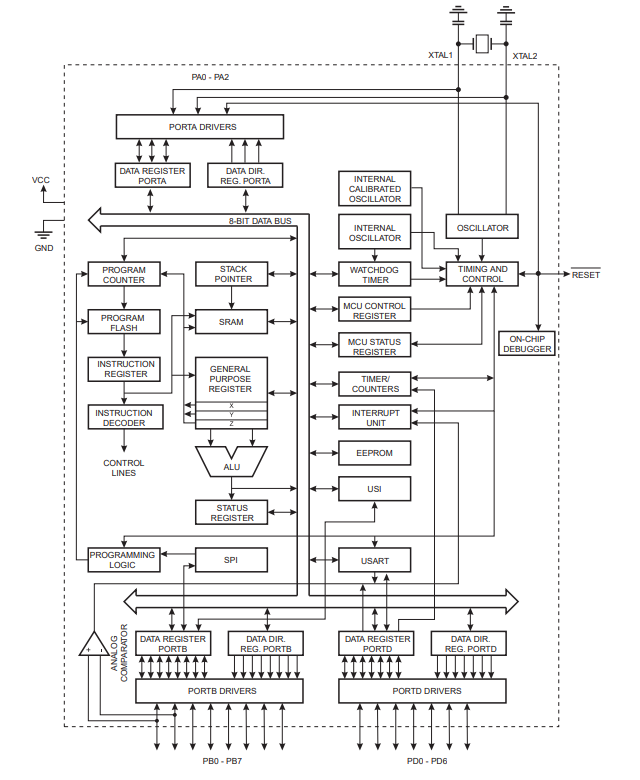
\includegraphics[width=0.9\textwidth]{imagenes/2.PNG}
    \caption{Diagrama de bloques de ATtiny4313. \cite{Microchip}.}
    \label{F:bloques}
    \end{figure}

\subsubsection{Diagrama de Pines}
En la figura \ref{F:pines} se observa el diagrama de pines para el microcontrolador ATtiny4313. 

\begin{figure}[H]
    \centering
    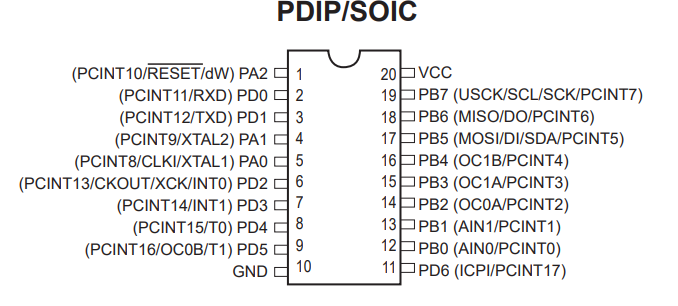
\includegraphics[width=1.0\textwidth]{imagenes/1.PNG}
    \caption{Diagrama de pines de ATtiny4313. \cite{Microchip}.}
    \label{F:pines}
    \end{figure}


    \newpage
\subsubsection{Caracter\'isticas El\'ectricas}
Las caracter\'isticas el\'ectricas del microcontrolador  ATtiny4313 se observan el la figura \ref{F:ELEC}. 

\begin{figure}[H]
    \centering
    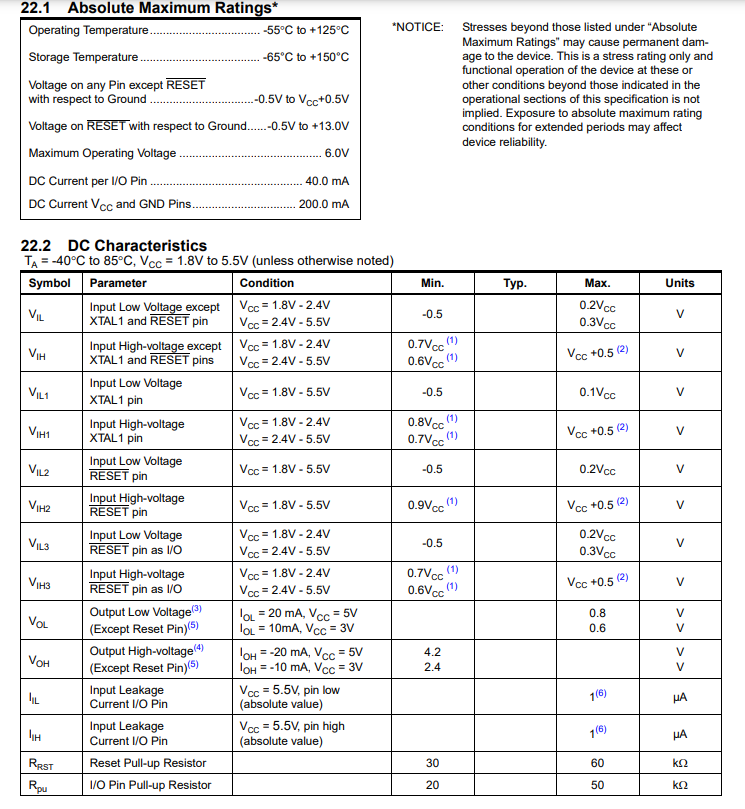
\includegraphics[width=1.0\textwidth]{imagenes/elec.PNG}
    \caption{Caracter\'isticas El\'ectricas del microcontrolador ATtiny4313. \cite{Microchip}.}
    \label{F:ELEC}
    \end{figure}


\subsection{Perif\'ericos Utilizados}
Los perif\'ericos en este laboratorio hacen referencia a los registros utilizados.
\subsubsection{Registro DDRB}
Se le conoce como \textit{PORTB}. Es el registro de configuraci\'on de los pines correspondientes al puerto B \cite{Microchip}. Su configuraci\'on se observa en la figura \ref{F:DDRB}

\begin{figure}[H]
    \centering
    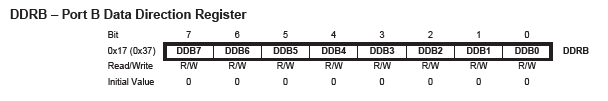
\includegraphics[width=1.0\textwidth]{imagenes/3.PNG}
    \caption{Registro DDRB. \cite{Microchip}.}
    \label{F:DDRB}
    \end{figure}
    
\subsubsection{Registro Puerto B}
Es un registro bidireccional, que se encarga de avisar al microcontrolador si el registro DDRB se encuentra encendido o apagado. Sus funciones alternativas se observan en las figuras \ref{F:B1} y \ref{F:B2}.

\begin{figure}[H]
    \centering
    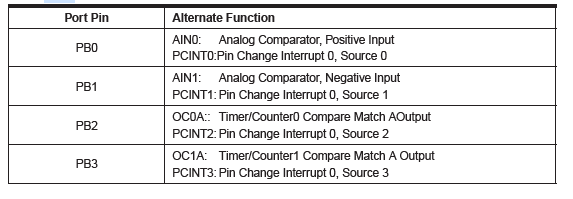
\includegraphics[width=1.0\textwidth]{imagenes/4.PNG}
    \caption{Registro Puerto B (1). \cite{Microchip}.}
    \label{F:B1}
    \end{figure}

\begin{figure}[H]
    \centering
    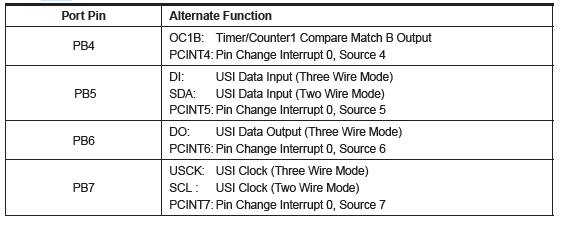
\includegraphics[width=1.0\textwidth]{imagenes/5.PNG}
    \caption{Registro Puerto B (2). \cite{Microchip}.}
    \label{F:B2}
    \end{figure}
    
\subsubsection{Registro GIMSK}
Se asocia con los eventos que detienen el flujo de instrucciones en un procesador, las interrupciones. Al ejecutar su funci\'on el procesador retoma sus tareas donde fueron interrumpidas \cite{Microchip}. Su configuraci\'on se observa en la figura \ref{F:GIM}.

\begin{figure}[H]
    \centering
    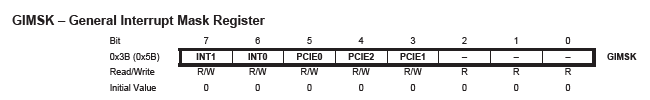
\includegraphics[width=1.0\textwidth]{imagenes/6.PNG}
    \caption{RegistrO GIMSK. \cite{Microchip}.}
    \label{F:GIM}
    \end{figure}

\subsubsection{Registro MCUCR}
Es un registro que controla las interrupciones externas. Revisa estas al detectar un flanco positivo o negativo. Su configuraci\'on general se observa en la figura \ref{F:MCU}.

\begin{figure}[H]
    \centering
    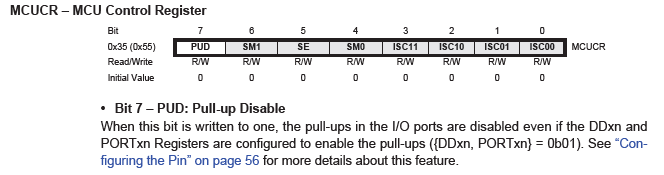
\includegraphics[width=1.0\textwidth]{imagenes/7.PNG}
    \caption{Registro MCUCR. \cite{Microchip}.}
    \label{F:GIM}
    \end{figure}


\subsubsection{Temporizadores}
El microcontrolador ATiny4314 tiene contadores para cuantificar el tiempo. Existen dos registros que afectan estos contadores al modificar su valor. El TIMSK activa interrupciones en el contador, y TCCR0B se habilita cuando hay una interrupci\'on. Su configuraci\'on se observa en la figura \ref{F:Temp}.

\begin{figure}[H]
    \centering
    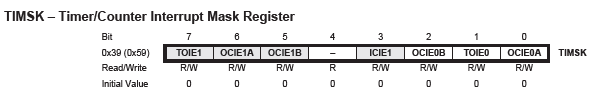
\includegraphics[width=1.0\textwidth]{imagenes/8.PNG}
    \caption{Temporizadores. \cite{Microchip}.}
    \label{F:Temp}
    \end{figure}

    


\subsection{Componentes Electr\'onicos Complementarios}
\subsubsection{LEDS de colores}
El diodo emisor de luz (LED por sus siglas en ingles) es un diodo que emite luz visible o invisible (infrarroja) cuando se energiza. Aun cuando la luz no es visible, los LED infrarrojos tienen numerosas aplicaciones donde la
luz visible no es un efecto deseable. Éstas incluyen sistemas de seguridad, procesamiento industrial, acoplamiento óptico controles de seguridad como abrepuertas de cochera y centro de entretenimiento domésticos, donde la luz infrarroja del control remoto es el elemento de control. \cite{boylestad}

\begin{figure}[H]
 \centering
  \subfloat[Símbolo esquemático LED]{
   \label{f:simbolo led}
    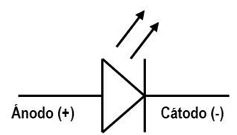
\includegraphics[width=0.3\textwidth]{imagenes/simbolo led.jpg}}
  \subfloat[Diodo LED]{
   \label{f:diodo led}
    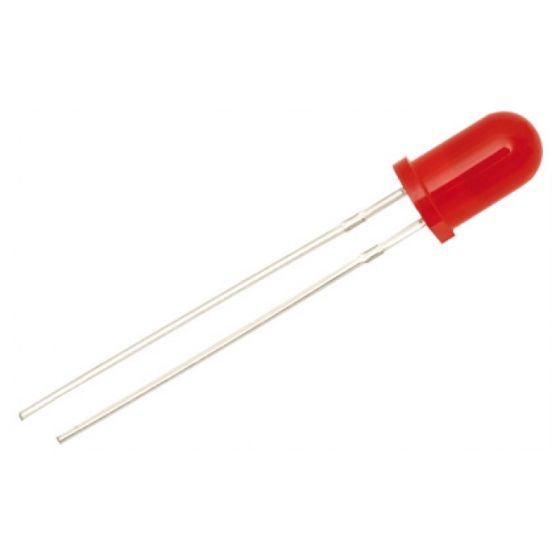
\includegraphics[width=0.3\textwidth]{imagenes/diodo led.jpg}}
 \caption{Diodo emisor de luz (elaboración propia)}
 \label{f:LED}
\end{figure}
\subsubsection{Resistores}
El elemento de circuito que se usa para modelar el comportamiento de resistencia a la corriente de un material es el resistor. Para efectos de fabricación de circuitos, los resistores suelen hacerse de aleaciones metálicas y compuestos de carbono. El símbolo
de circuito del resistor se presenta en la figura \ref{f:simbolo resistor}, donde R significa la resistencia del resistor. El resistor es el elemento pasivo más simple. \cite{alexander}

\begin{figure}[H]
 \centering
  \subfloat[Símbolo esquemático resistor]{
   \label{f:simbolo resistor}
    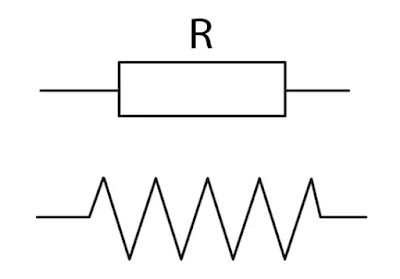
\includegraphics[width=0.3\textwidth]{imagenes/equema resistor.png}}
  \subfloat[Resistor]{
   \label{f:resistor real}
    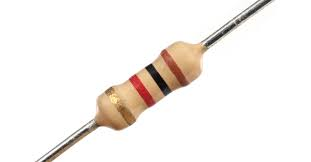
\includegraphics[width=0.3\textwidth]{imagenes/resistor.jpeg}}
 \caption{Resistor (elaboración propia)}
 \label{f:resistor}
\end{figure}

\subsubsection{Bot\'on}
Los botones son un tipo de interruptor donde permiten o detienen el flujo de corriente solo cuando están presionados. Existen 2 tipos, Normalmente Cerrado (NC) y Normalmente Abierto). Para el primer tipo, presionar el botón hará que el circuito se abra por un lapso de tiempo y luego vuelva a cerrar. Para el segundo tipo ocurre lo contrario, presionar el botón hará que se cierre el circuito y haya flujo de corriente, después de cierto tiempo se abrirá de nuevo \cite{botondef}. Los interruptores en general rebotan cuando se abren o se cierran, por lo que se debe tomar en cuenta a la hora de construir el circuito. Una forma de resolverlo es mediante la agregación de un retraso en el código. Otra forma es mediante la adición de un capacitor, donde la capacitancia se calcula con la resistencia y la constante de tiempo deseada.

\begin{figure}[H]
 \centering
  \subfloat[Símbolo esquemático botón normalmente abierto]{
   \label{f:boton na}
    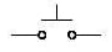
\includegraphics[width=0.3\textwidth]{imagenes/boton na.png}}
  \subfloat[Símbolo esquemático botón normalmente cerrado]{
   \label{f:boton nc}
    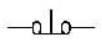
\includegraphics[width=0.3\textwidth]{imagenes/boton nc.png}}
    \subfloat[Botón]{
   \label{f:boton}
    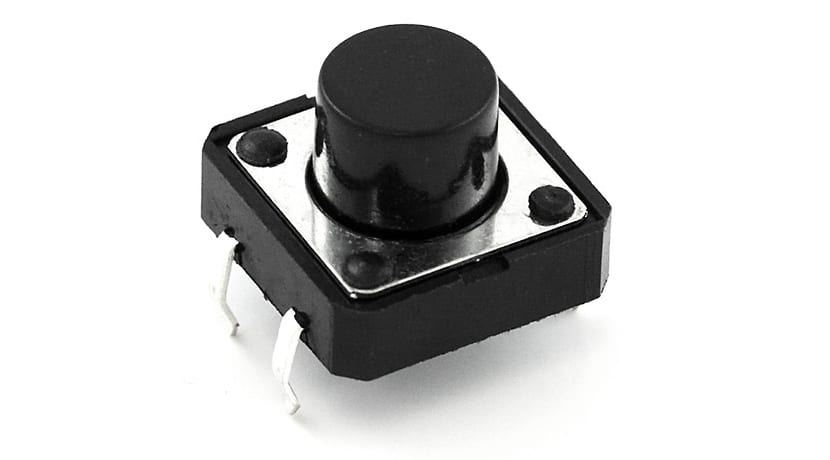
\includegraphics[width=0.3\textwidth]{imagenes/pulsador.jpg}}
 \caption{Botón (elaboración propia)}
 \label{f:pulsador}
\end{figure}

\subsection{Diseño}
El diseño a realizar esta basado en la figura \ref{F:semaforo}, la cual consiste en un semáforo vehicular, el cual se estará omitiendo la luz amarilla; y también dos semáforos peatonales en cada extremo de la calle. Se añaden dos botones, uno por semáforo peatonal, para que pueda ser activado desde cualquier extremo de la vía. El circuito a simular se encuentra en la figura \ref{F:circuito}.

\begin{figure}[H]
    \centering
    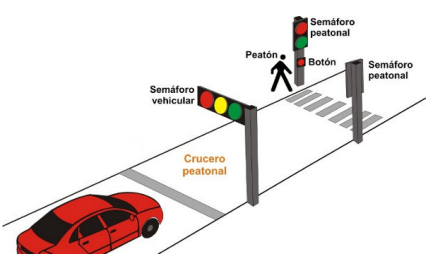
\includegraphics[width=0.7\textwidth]{imagenes/semaforo.png}
    \caption{Semáforo vehicular y peatonal.}
    \label{F:semaforo}
\end{figure}

Los diodos a utilizar para simular las luces de los semáforos deben cumplir las características de tener una tensión de polarización directa menor a 2.5 V y una corriente de polarización directa menor a 25 mA. Usando las especificaciones eléctricas de los diodos LED's ($V_{F}=2\:V$ cuando $I_{F}=20\:mA)$, se calcula el valor de las resistencias de protección para los LED's usando la fórmula \eqref{eq:RP}, y utilizando $V_{DD}=5\:V$ y según la hoja de datos del fabricante la tensión de salida en alto de los pines está dada por $V_{OH}=V_{DD}-0.7\:V$:

\begin{equation}
    R = \frac{V_{OH}-n\times V_{F}}{I_{F}}
    \label{eq:RP}
\end{equation}

Por lo que para el grupo 1 se obtiene lo siguiente:
\begin{equation}
    R = \frac{(5-0.7-2)\:V}{20\:mA} = 115\:\Omega
\end{equation}

Para utilizar valores comerciales se utilizaran dos resistencias en serie una de $100 \Omega$ y otra de $15 \Omega$. Sabemos que la fórmula de la potencia para un resistor es:
\begin{equation}
    P_{R} = I^{2}R = \frac{V^{2}}{R}
\end{equation}

Como tenemos dos valores de resistencia, su potencia máxima es:
\begin{align}
    P_{100\:\Omega} &= (20\:mA)^2\cdot100\:\Omega = 0.04\:W \\
    P_{15\:\Omega} &= (20\:mA)^2\cdot15\:\Omega = 0.006\:W
\end{align}

Cuando se pulsa un botón, la señal que emite no es completamente constante, ya que suele presentar lo que se denomina "rebote". Este fenómeno se origina debido a pequeñas interrupciones en el contacto entre los componentes internos del botón. Esto puede resultar en un problema, ya que los rebotes pueden generar lecturas incorrectas en el sistema. Para solucionar este inconveniente en el diseño del circuito, se incorporó un filtro pasivo.

Dado que la entrada del circuito es de corriente continua (DC) y no es necesario filtrar un rango específico de frecuencias, se optó por seleccionar los valores de los componentes del filtro de manera arbitraria. Esto implicó utilizar un condensador de $100 p$F en conjunto con dos resistencias de $100 \Omega$ cada una.
\begin{equation}
    \tau = R\cdot C=200\cdot 100=20 ns
\end{equation}


El intervalo de tiempo resultante es lo suficientemente amplio como para eliminar cualquier distorsión en la señal de entrada causada por el rebote del botón, pero al mismo tiempo, es lo bastante breve como para que el usuario no perciba ningún efecto adverso.

\begin{figure}[H]
    \centering
    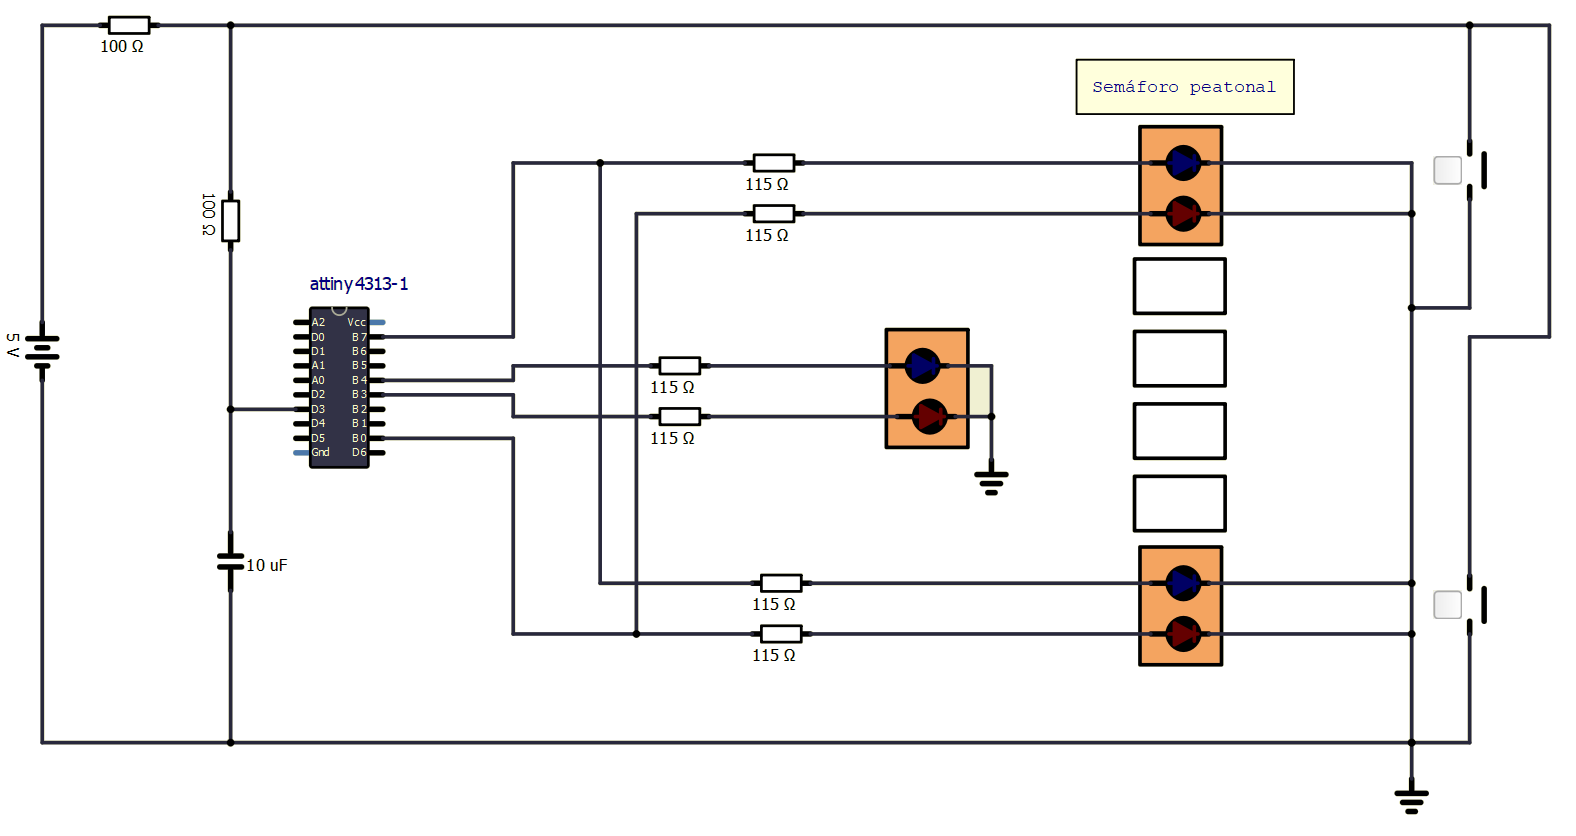
\includegraphics[width=0.9\textwidth]{imagenes/circuito semaforo.jpeg}
    \caption{Esquemático de simulación de un semáforo. (Elaboración propia).}
    \label{F:circuito}
    \end{figure}

\subsection{Lista de componentes y precios}
En la tabla \ref{T:componentes} se observa la lista de componentes a utilizar para la implementaci\'on del laboratorio. 

\begin{table}[H]
        \centering
        \begin{tabular}{| m{4cm} | m{4cm} |  m{4cm} | }
          \hline
          \textbf{Componente} &  \textbf{Cantidad} & \textbf{Precio} \\
        \hline 
        ATiny4313 & 1 & ₡710\\
        \hline
        Resistencia 100\ohm & 8 & ₡2392\\
         \hline
        Resistencia 15\ohm & 6 & ₡1794\\
         \hline
         LED & 6 & ₡158\\
         \hline
         Capacitor  & 1 &  ₡99 \\
         \hline
         Bot\'on & 2 & ₡178 \\
         \hline
         
         
           \end{tabular}
        \caption{Lista de componentes basada en Teltron CR. (Elaboración propia). }
        \label{T:componentes}
    \end{table}

\section{Desarrollo/An\'alisis de resultados}


\subsection{Diseño Lógico}
Se utiliza una estructura llamada FSM para definir los miembros que componen cada estado de la máquina. Cada estado tiene un puntero a una función de salida y un tiempo de duración.

El código realizado define cinco estados para el cruce de semáforos presentes en la tabla \ref{T:estados}. Cada estado representa una fase específica en el funcionamiento del semáforo. La función timer\_setup() configura el temporizador del microcontrolador para generar interrupciones periódicas. Esto se utiliza para medir el tiempo en cada estado.

Se definen funciones para controlar la activación de los LED's en cada estado. Por ejemplo, paso\_vehicular\_ON() enciende la luz verde del semáforo vehicular y apaga la luz roja del semáforo peatonal. Las funciones paso\_vehicular\_WARNING(), luces\_OFF(), paso\_peatonal\_ON() y paso\_peatonal\_WARNING() hacen lo mismo para otros estados. En la figura \ref{F:maquina de estados} se logra observar la logica utilizada para realizar este diseño.

El bucle principal en main() implementa la lógica de la máquina de estados. Se utiliza una estructura para cambiar entre estados y llamar a las funciones de salida correspondientes. La máquina de estados avanza según el tiempo y las señales de los botones. Se utiliza una interrupción del temporizador (TIMER0\_OVF\_vect) para gestionar el tiempo y cambiar los estados según el tiempo definido en cada estado. Esta interrupción ocurre periódicamente y se usa para implementar el temporizador de 10 segundos y el contador de 1 segundo.

\begin{table}[H]
        \centering
        \begin{tabular}{| m{3cm} | m{5cm} |}
          \hline
          \textbf{Estado} &  \textbf{Definición}  \\
        \hline 
        A & Paso vehicular ON \\
        \hline
        B & Paso vehicular WARNING \\
         \hline
         C & Luces OFF\\
         \hline
         D  & Paso peatonal ON  \\
         \hline
         E & Paso peatonal WARNING  \\
         \hline
        \end{tabular}
        \caption{Tabla de estados. (Elaboración propia). }
        \label{T:estados}
\end{table}

\begin{figure}[H]
    \centering
    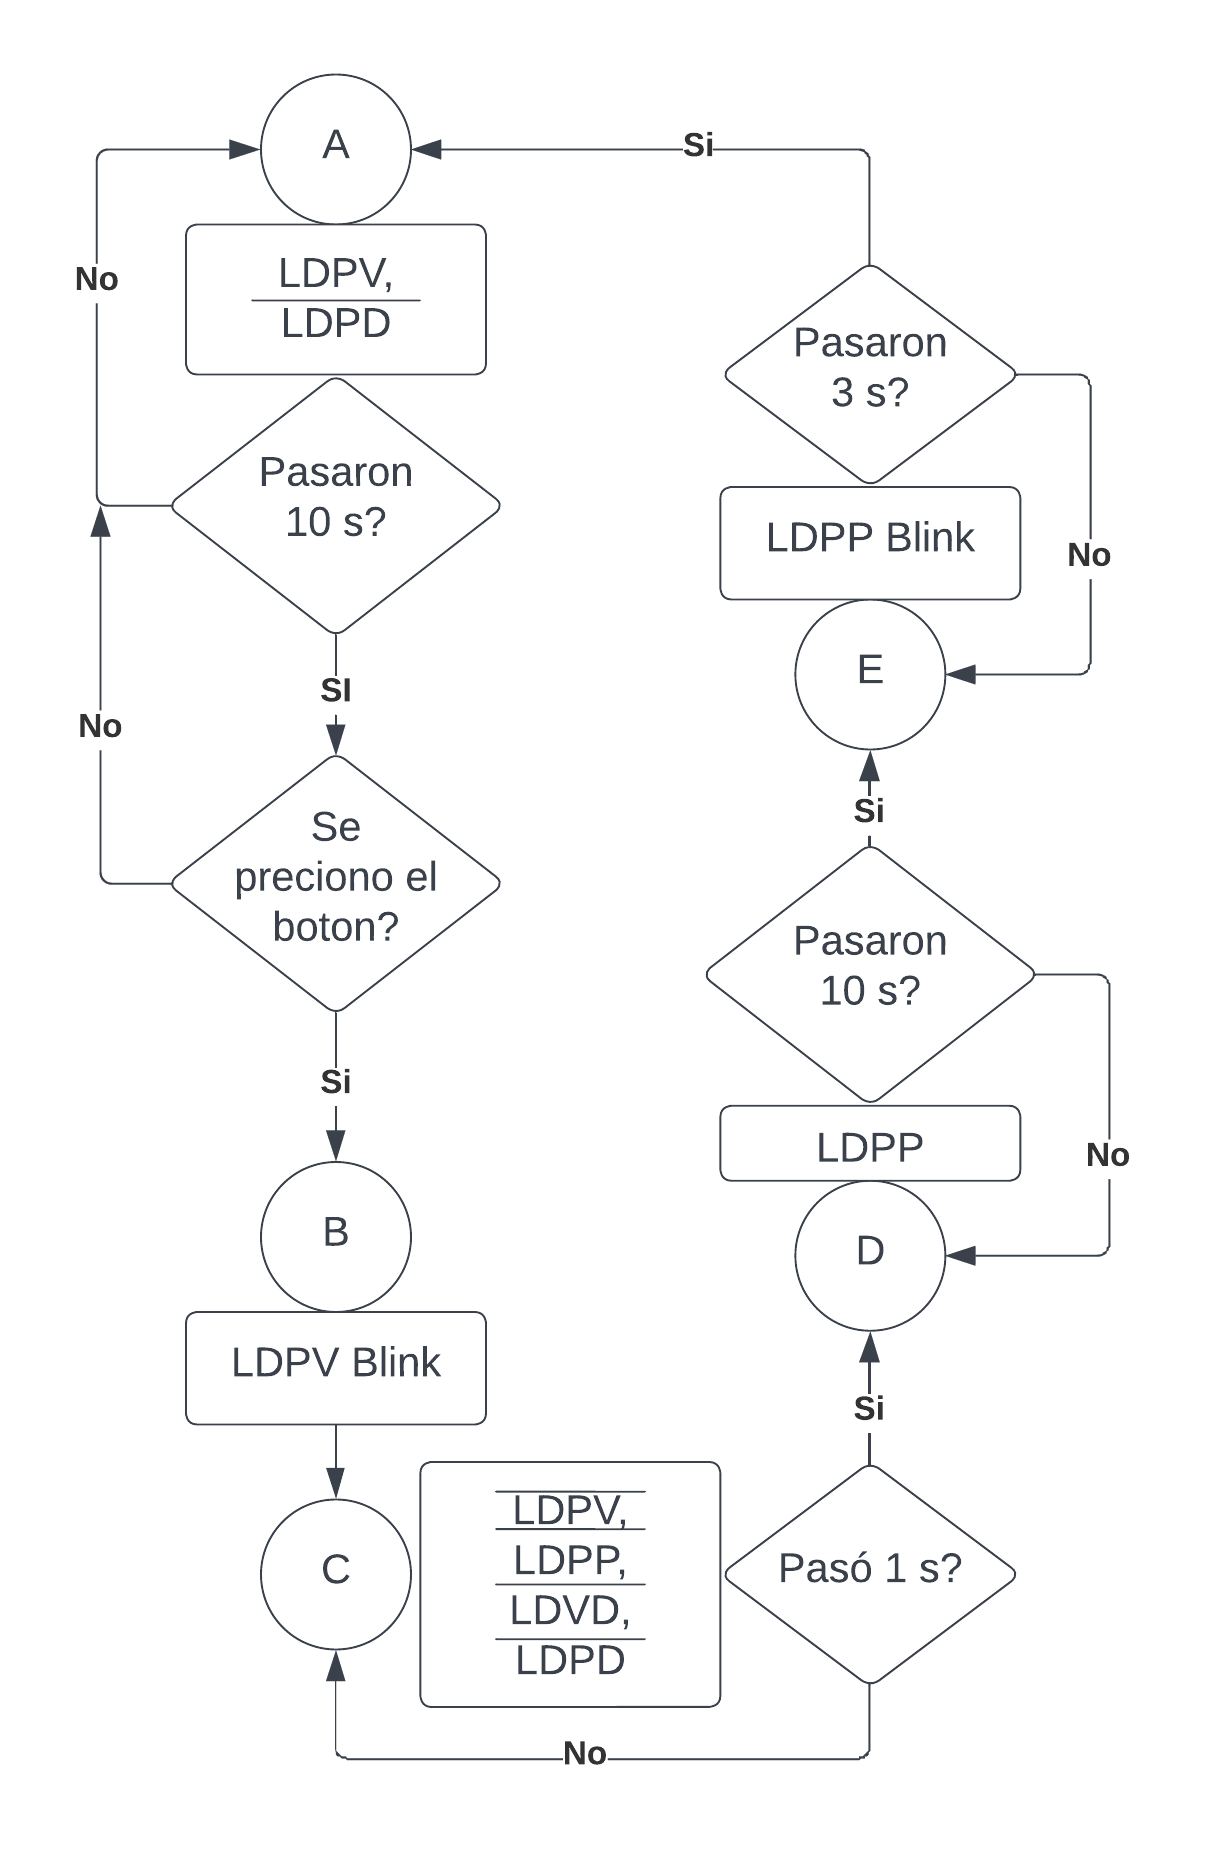
\includegraphics[width=0.5\textwidth]{imagenes/maquina de estados.png}
    \caption{Maquina de estados semáforo. (Elaboración propia).}
    \label{F:maquina de estados}
\end{figure}




\subsection{Resultados}
En esta sección se presentan los resultados obtenidos al simular el circuito. Se presentan capturas del momento en el que los vehículos deben pasar mientras que los peatones se encuentran detenidos, también se presenta el caso contrario en que los peatones pasan y los vehículos deben permanecer quietos.

Se logra observar en las figuras \ref{F:vehiculos} y \ref{F:peatones} las corrientes y tensiones de los LED's, los cuales cumplen con las especificaciones de su hoja de datos para el buen funcionamiento. No se pueden incluir imágenes de las señales de "Warning" de cada semáforo ya que no se lograría apreciar cuando se encienden y se apagan, pero es posible observar en la simulación.
\begin{figure}[H]
    \centering
    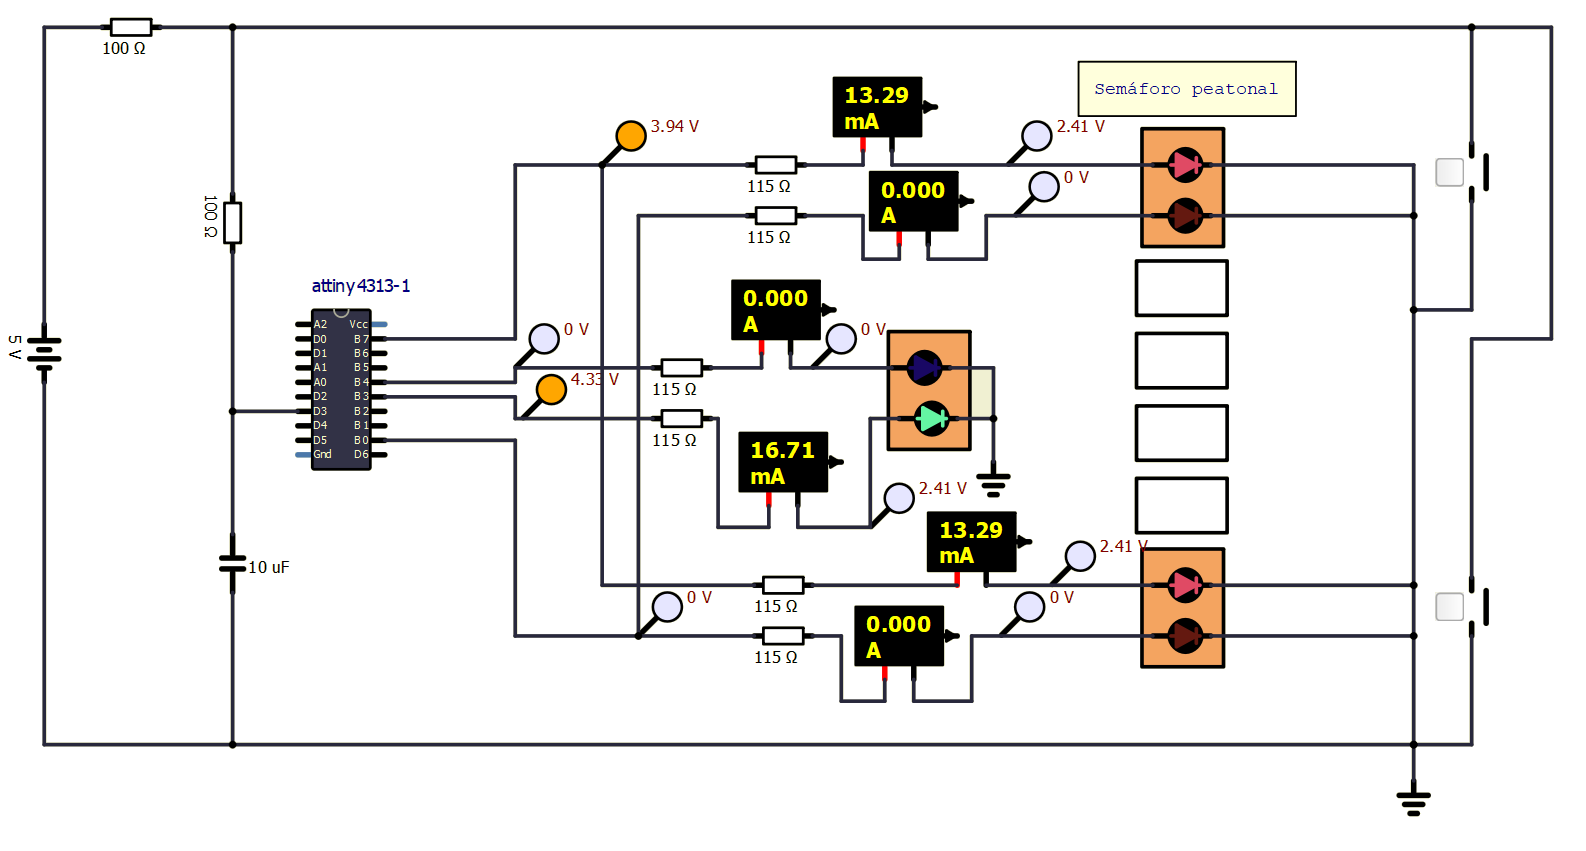
\includegraphics[width=0.9\textwidth]{imagenes/paso vehiculos.jpeg}
    \caption{Semáforo vehicular en posición de paso. (Elaboración propia).}
    \label{F:vehiculos}
\end{figure}

\begin{figure}[H]
    \centering
    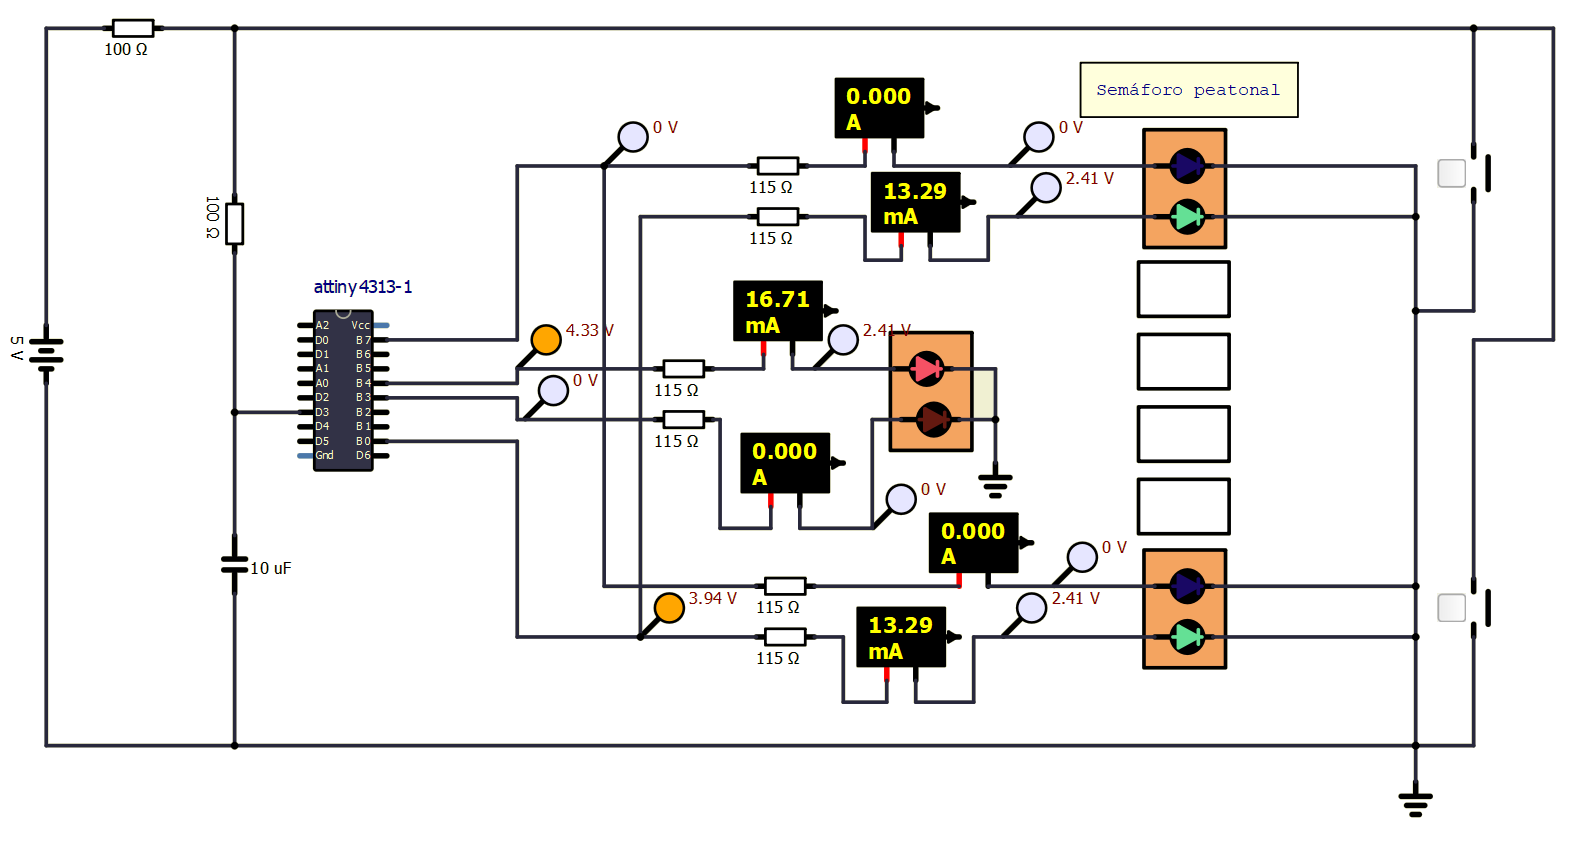
\includegraphics[width=0.9\textwidth]{imagenes/paso peatones.jpeg}
    \caption{Semáforo peatonal en posición de paso. (Elaboración propia).}
    \label{F:peatones}
\end{figure}

\subsection{Guía de ejecución}
A continuación se presenta una guía de como ejecutar el programa, cabe resaltar que esta simulación fue realizada en el sistema operativo Windows 11, empleando WSL ,no obstante los pasos no deberían variar respecto a otros sistemas operativos.
\begin{enumerate}
    \item Clonar el repositorio \url{https://github.com/joseeras98/Laboratorio-2.git}.
    \item Moverse a la carpeta src.
        \begin{minted}{bash}
            cd src
        \end{minted}
        En esta carpeta encontrara el código fuente, un archivo respectivo al simulador, y un Makefile.
    \item Ejecutar el archivo Makefile con el siguiente comando:
        \begin{minted}{bash}
            make
        \end{minted}
    \item Abrir manualmente el simulador SimulIDE.
    \item Cargar el archivo con extensión .simu.
    \item En el controlador ATtiny4313, hacer click izquierdo y cargar el firmware, el cual tiene extensión .hex y se crea automáticamente en el paso número 3.
    \item Correr la simulación.
\end{enumerate}


\section{Conclusiones y recomendaciones}
En esta secci\'on se describen los conclusiones y las recomendaciones del laboratorio:

\begin{itemize}
    \item Para el uso correcto de los pines, se recomienda leer la hoja del fabricante con detenimiento en los puntos importantes. 
    \item Se sugiere explicar el funcionamiento de los microcontroladores que entran dentro del marco de este curso mediante videos, o material menos est\'atico con respecto a una presentaci\'on. 
    \item Se concluye que las técnicas de interrupción es un método mas eficiente para realizar cambios de estado en un sistema electrónico. Ya que ses aprovechar las funciones de las que dispone el microcontrolador.
\end{itemize}


\newpage

\bibliographystyle{unsrt}
\bibliography{bibliografia.bib}
\newpage
%\begin{thebibliography}{9}
%\bibitem{1} Microchip. PIC12F683. Disponible en l\'inea, 
%accesado el 30 de Agosto de 2023. url: \url{https://ww1.microchip.com/downloads/en/devicedoc%/41211d\_.pdf}.


%\end{thebibliography}

%\section{Anexos}
%\includepdf[pages=-]{ATtiny2313.pdf}
\section{Anexos}
\includepdf[pages=-]{./Documentos/ATtiny2313.pdf}
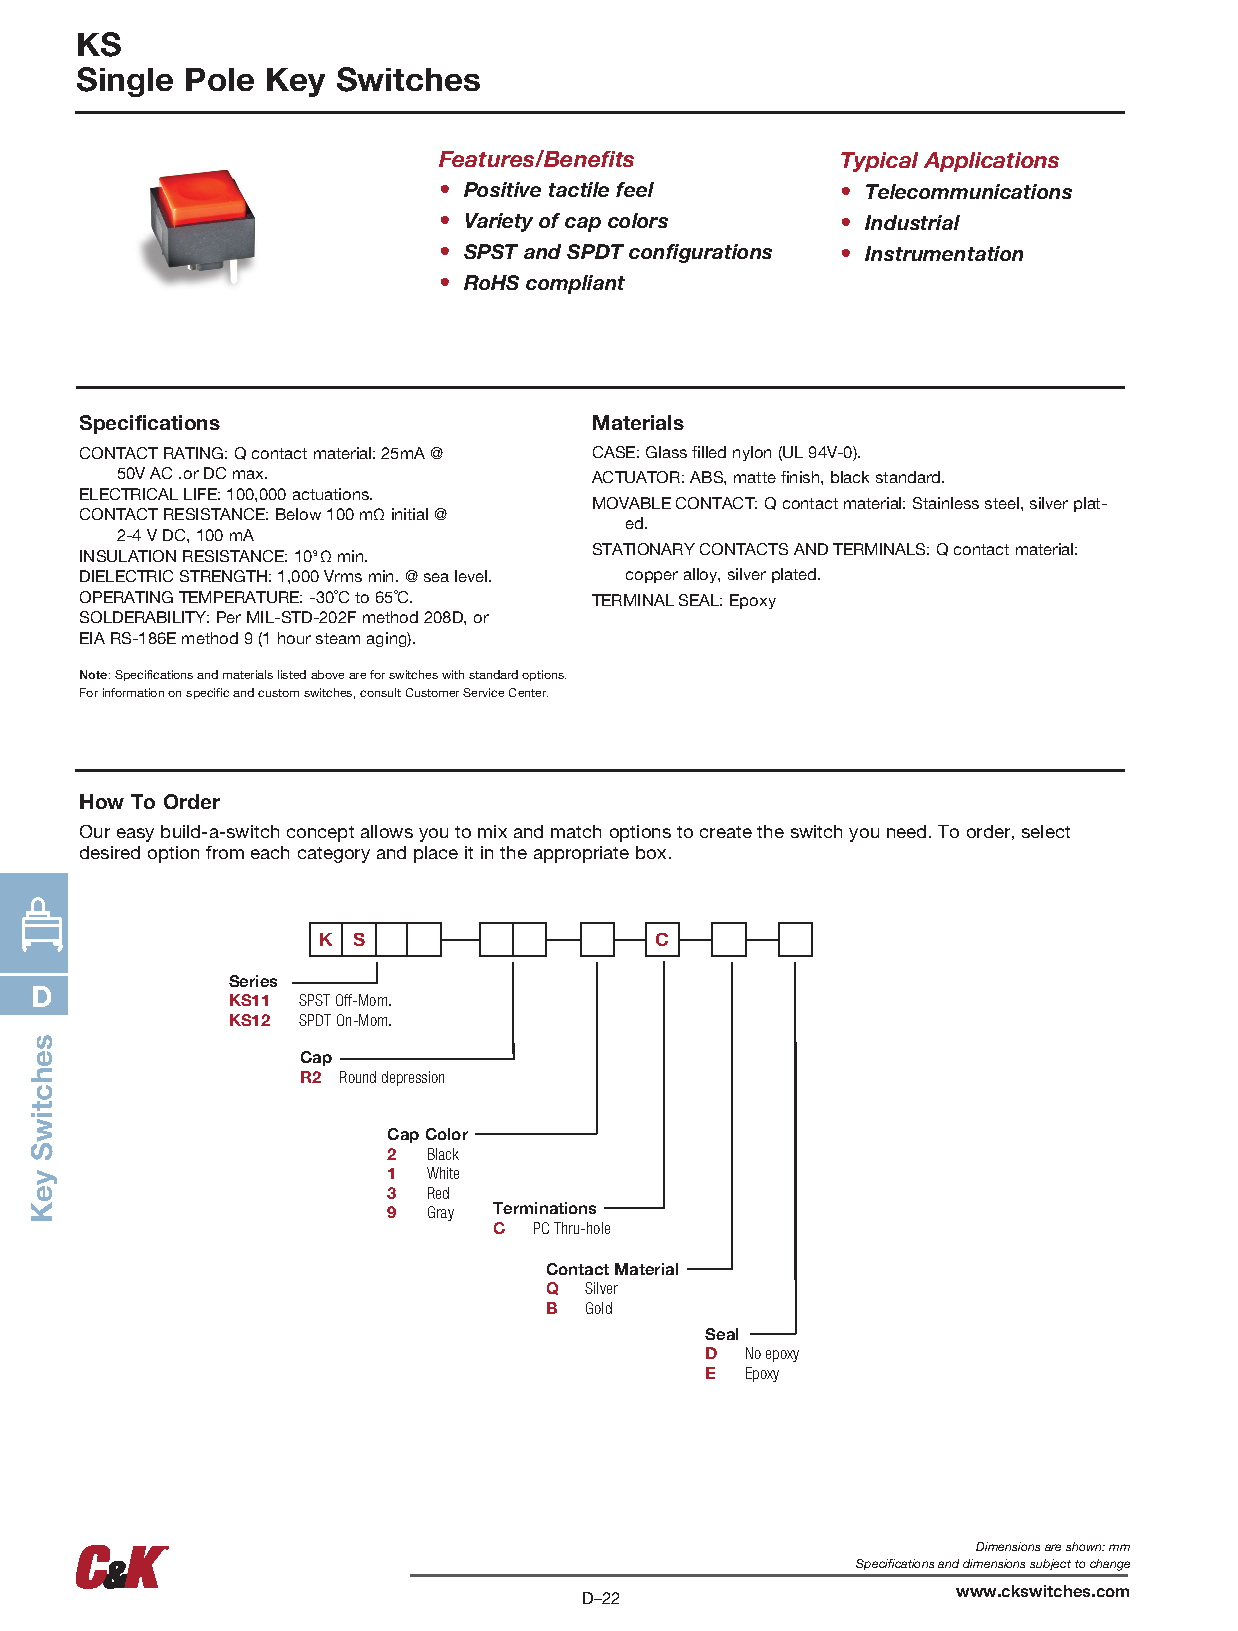
\includepdf[pages=-]{./Documentos/boton.pdf}
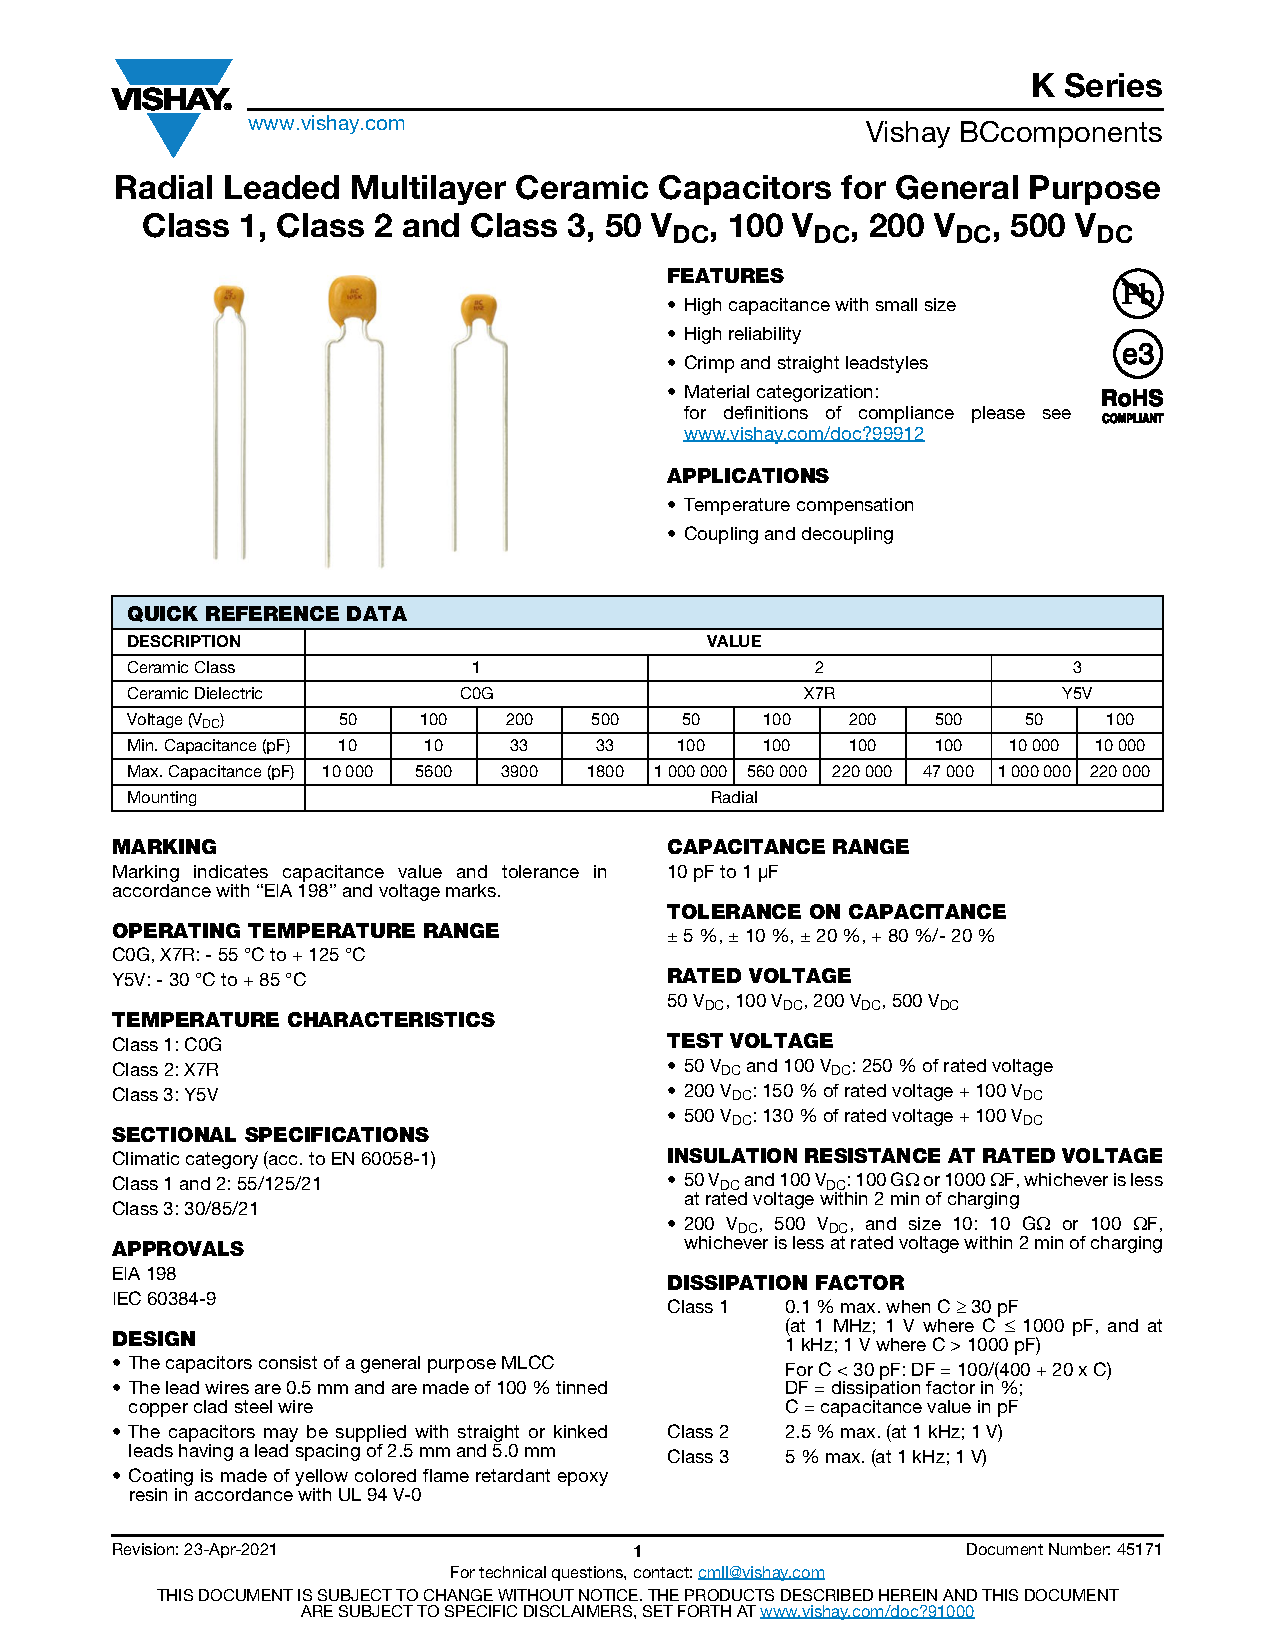
\includepdf[pages=-]{./Documentos/capacitor.pdf}
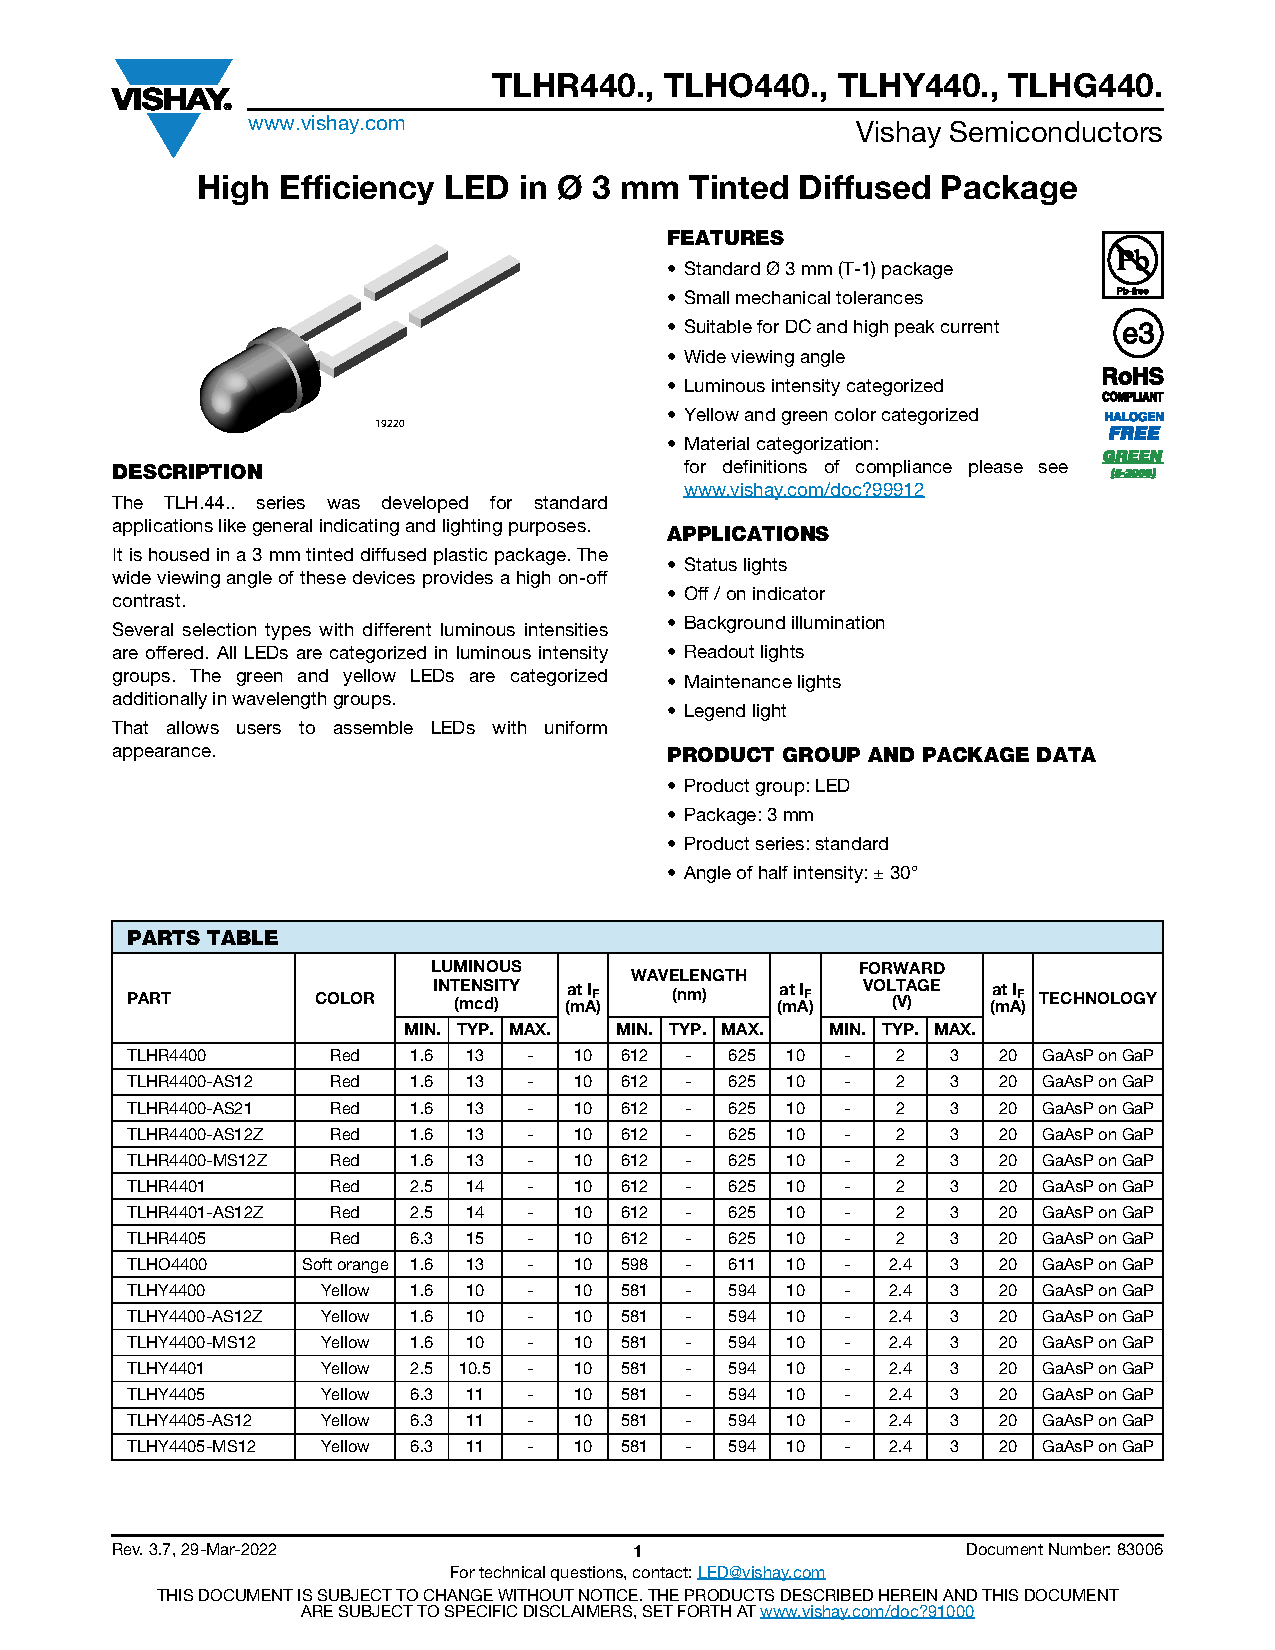
\includepdf[pages=-]{./Documentos/led.pdf}
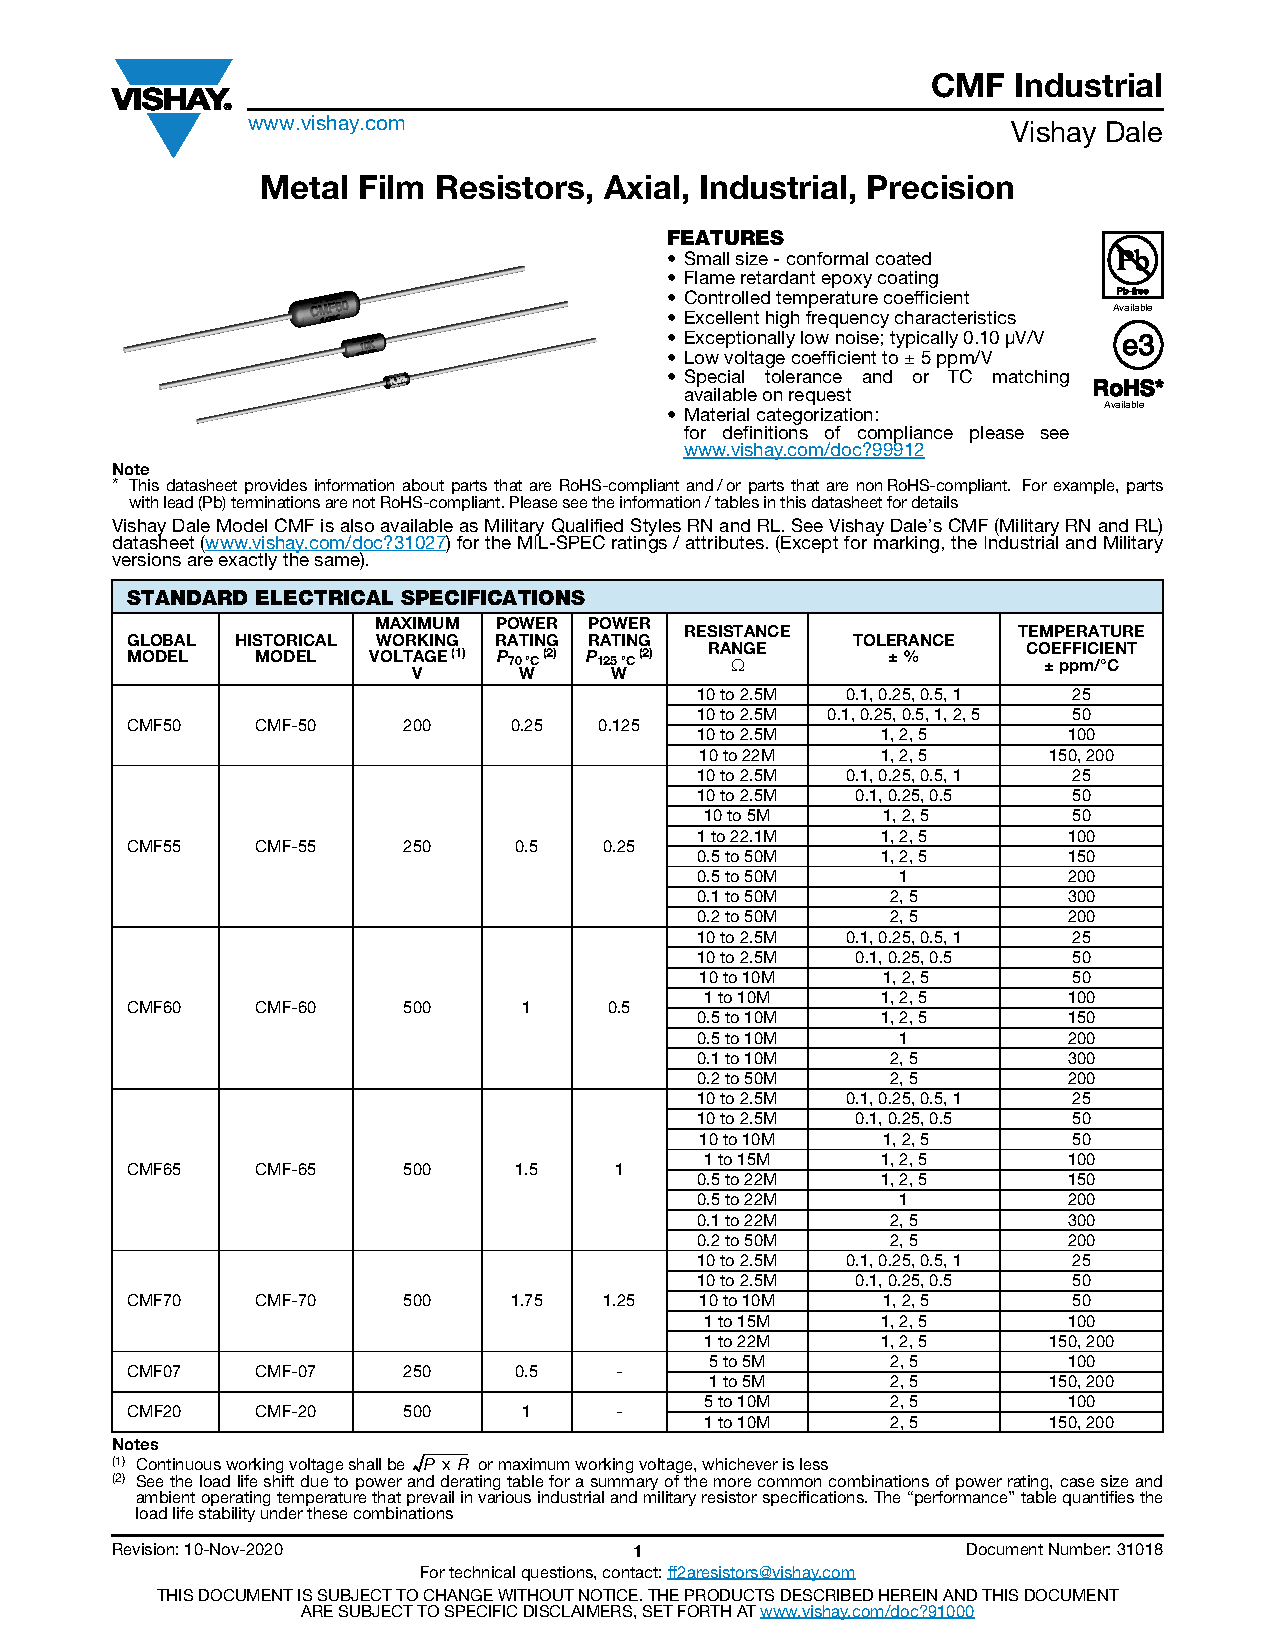
\includepdf[pages=-]{./Documentos/resistencia.pdf}


%%%%%%%%%%%%%%%%

%%%%%%%%%%%%%%
\end{document}
%%%%%%%%%%%%%%

%%%%%%%%%%%%%%%%%%%%%%%%%%%%%%%%%%%%%%%%%%%%%%%%%
% copyleft | Fabián Abarca Calderón, diciembre 2011
% Se autoriza su uso, modificación y reproducción
%%%%%%%%%%%%%%%%%%%%%%%%%%%%%%%%%%%%%%%%%%%%%%%%% 


